\documentclass{beamer}

\usepackage{amsfonts, amsmath, amssymb}
\usepackage{tikz}

\usetheme{Marburg}
\usecolortheme{orchid}
\usefonttheme{professionalfonts}



\begin{document}

    % Cayley's generating function for rooted treees.
    \begin{frame}{Cayley's generating function for rooted trees}
    \begin{figure}
        \centering
        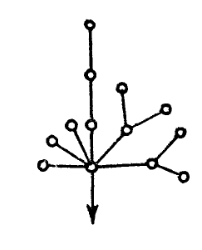
\includegraphics[scale=0.5]{images/rooted-tree.png}
        \caption{A rooted tree}
        \label{fig:enter-label}
    \end{figure}
        \begin{definition}
            A \emph{tree} is a graph consisting of vertices and edges 
            but contains no closed path. A \emph{rooted tree} is a tree with one distinguished vertex called the \emph{root}. A non-root vertex is called a \emph{knot}.
        \end{definition}
    
    \end{frame}

    \begin{frame}
        \begin{figure}
        \centering
        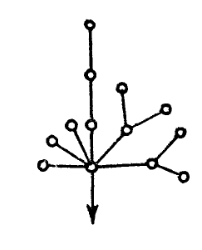
\includegraphics[scale=0.7]{images/rooted-tree.png}
        \label{fig:enter-label}
    \end{figure}
    \begin{block}{Question}
        How many rooted trees with $n$ knots?
    \end{block}
    \pause
     Let there be $T_n$ such trees, we look for a generating function with 
    $T_n$ as coefficient.
    \end{frame}
    
    \begin{frame}{A visual proof}{Cayley's generating function for $T_n$}
    
    \begin{align*}
        & T_1x + T_2 x^2 + T_3 x^3 +\cdots \\
        =\,  & x(1-x)^{-T_1}(1-x^2)^{-T_2}(1-x^3)^{-T_3}\cdots
    \end{align*}
    \end{frame}

    \begin{frame}{Taking apart the tree}
        \begin{figure}
            \centering
            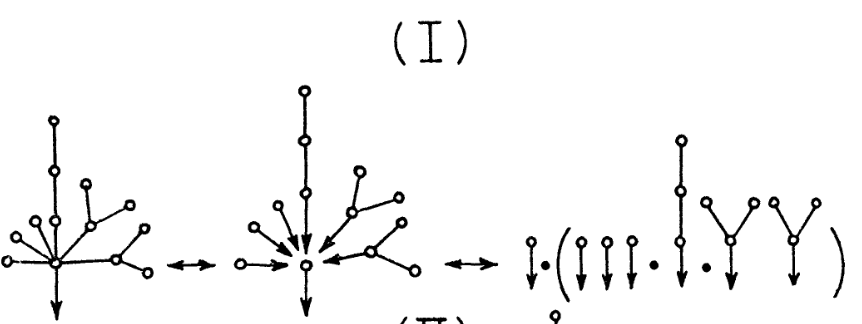
\includegraphics[scale=0.6]{images/tree1.png}
            \label{fig:enter-label}
        \end{figure}
    \pause
    Combinatorial insight: a rooted tree consists of \underline{the root} +  
    \begin{enumerate}
        \item some number of $1$-trees
        \item some number of $2$-trees
        \item etc.
    \end{enumerate}
    where the total number of knots add up to $n$.
    \end{frame}

    \begin{frame}{Important Observation}

        \begin{figure}
            \centering
            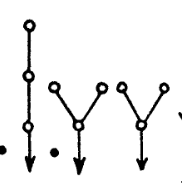
\includegraphics{images/tree2.png}
            \caption{A $3$-tree can be chosen $T_3$ different ways!}
            \label{fig:enter-label}
        \end{figure}
    \end{frame}

    \begin{frame}{Making choices by multiplication}
        \begin{figure}
            \centering
            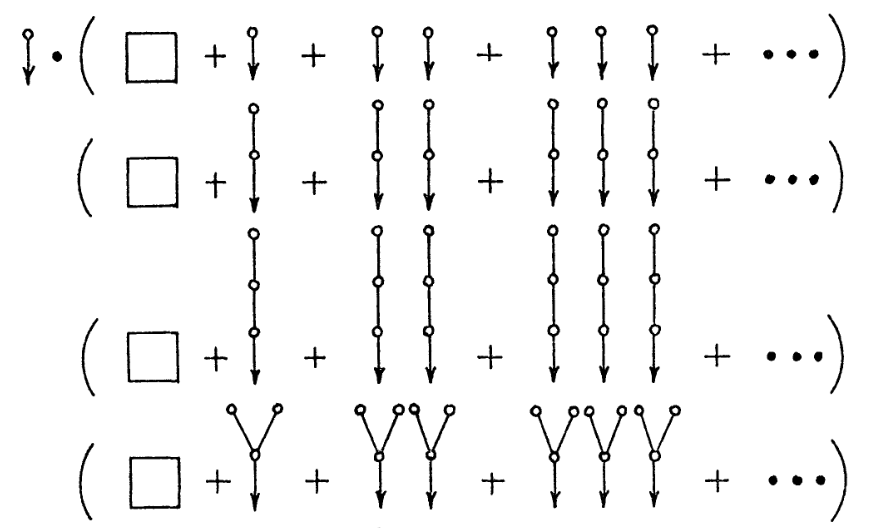
\includegraphics[scale=0.5]{images/tree3.png}
            \caption{Infinitely many rows: $T_k$ rows for $k$-trees}
            \label{fig:enter-label}
        \end{figure}
        Insight: when you expand this product you are actually making choices
    \end{frame}

    \begin{frame}{Visual generating function}
        \begin{figure}
            \centering
            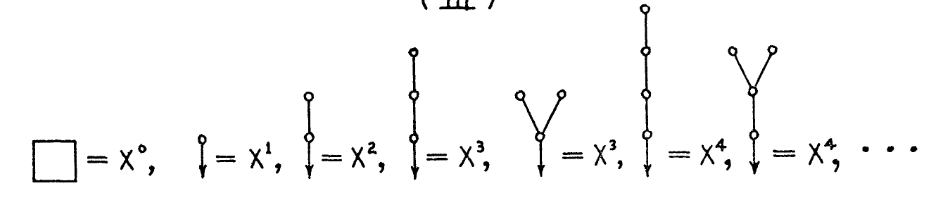
\includegraphics[scale=0.6]{images/tree5.png}
            \caption{convert pictures into algebra}
            \label{fig:enter-label}
        \end{figure}
    \begin{align*}
        & T_1x + T_2 x^2 + T_3 x^3 +\cdots \\
        =\,  & \underbrace{x}_{\text{this $x$ accounts for the root}}(1-x)^{-T_1}(1-x^2)^{-T_2}(1-x^3)^{-T_3}\cdots
    \end{align*}
    \end{frame}

    \begin{frame}{Fun Fact}
Cayley also has a theorem for the number of \underline{labeled} trees.

    \begin{figure}
        \centering
        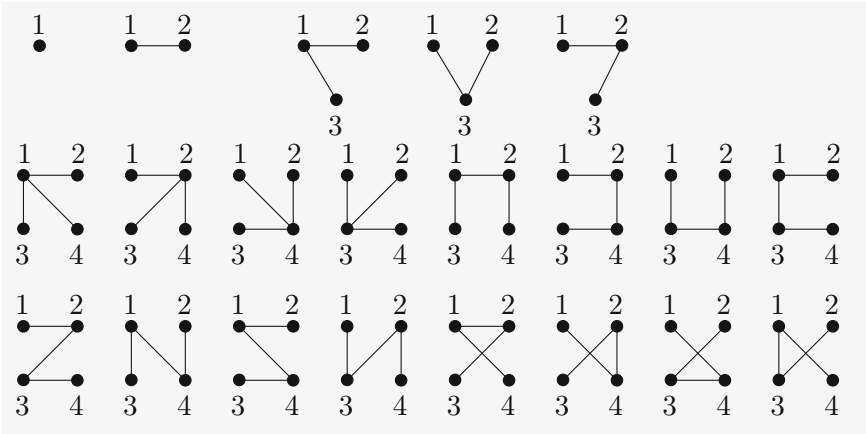
\includegraphics[scale=0.5]{images/numbered-trees.png}
        \caption{There are $n^{n-2}$ labeled trees on $n$ vertices!}
        \label{fig:enter-label}
    \end{figure}
    \pause
    And even one for rooted forest (a collection of $k$ disconnected trees with total $n$ vertices)
    $$\mathcal{F}_{n,k}=\binom{n}{k}kn^{n-1-k}$$
    \end{frame}
\end{document}

